\documentclass{article}
\usepackage[utf8]{inputenc}
\usepackage[margin=0.75in]{geometry}
\usepackage{enumitem}
\usepackage{graphicx}
\usepackage{hyperref}
\usepackage{soul}
\graphicspath{ {./images/} }
\begin{document}
	\begin{center}
    	% MAKE SURE YOU TAKE OUT THE SQUARE BRACKETS
        \topskip 0pt
        \vspace*{\fill}
    		\LARGE{\textbf{Software Design Specification}} \\
            \vspace{1em}
            \Large{Engineering Admission Cutoff Learning System} \\
            \vspace{1em}
            \normalsize\textbf{Nikou Kalbali, Maryyam Niazi, Jan Ollers, Yaminah Qureshi} \\
            \normalsize{kalbaln@mcmaster.ca, niazim3@mcmaster.ca, qureshiy@mcmaster.ca, ollersjp@mcmaster.ca} \\
            \vspace{1em}
            \normalsize{Supervisor: Dr. Franek} \\
            \vspace{1em}
            \normalsize{Group 2} \\
    \vspace*{\fill}
	\end{center}
	
	\newpage
    \begin{normalsize}
    \tableofcontents
    \newpage
    
    % a lot of this section is the exact same as the requirement spec we handed in, probably should look at refining/improving/changing it
    \section{Introduction}
        \subsection{Background}
        A typical university admission process in Ontario takes two steps.
        The first step consists of determining a cutoff threshold to define a subset of all applicants that will be extended an offer if their grade average is not below the cutoff.
        Some of the offerees become acceptees, while others do not. The second step involves determining the number of applicants the university should be preparing to welcome to their institution and programs. \newline
        \indent In this process, determining an ideal cutoff threshold such that the acceptees set is of a specific size with some small tolerance is difficult.
        If the threshold is undervalued, the number of offerees is overshot, typically leading to an acceptees set that is too large and costs the university financial and space issues from having to deal with too many students.
        If the threshold is overvalued, the number of offerees will be undershot, resulting in a set of acceptees that is too small and costing the university opportunities for revenue and funding from tuition fees and government support. \newline
        \indent This project will use at least two different machine learning approaches trained on previous years of applicant data and their acceptance of offers to an Ontario university to tackle the problem of determining ideal cutoff thresholds for new applicant data pools based on the learned patterns.
    
        \subsection{Purpose}
        The purpose of this document is to define the software design of the outlined system.
        
        \subsection{Statement of Goals}
        The system will be used for determining cutoff thresholds for two programs at an Ontario university. \newline
        \indent By taking in applicant information from the current admission cycle and using information from previous admission cycles, the cutoff thresholds will be estimated to obtain an ideal number of offerees, such that the predicted number of acceptees should be as close to the target seat cap as possible.
        
        \subsection{Users}
        The primary intended users of the system are the admissions committees for Ontario universities. The system may be used as an analysis tool to help them evaluate and/or improve their current admissions process. Furthermore, if we can expand the system and make it applicable to other university program admissions, the admissions committees of these programs will serve as secondary users.

    \section{Functional Description}
        \subsection{Data}
        The system will be developed using applicant pool data from 8 years of admission cycles for two programs at an Ontario university. We describe some nuances related to the data in the following section.
        
        \subsubsection{Extracting Offeree Data}
        \label{cutoffMetDataCleaning}
        As our system will be predicting whether or not a student accepted an offer, we will only consider students that met the cutoff average for their application year for the University programs in question. This will be done by determining the GPA cutoff threshold for each admissions year and extracting the data for students that met this threshold.
        \subsubsection{Applicant Features}
        Our data contains multiple attributes about applicants in an admissions cycle, however, we only consider the following attributes of each student and will refer to these as \textbf{features}:
        \begin{enumerate}
            \item \textbf{Applicant GPA} - 
                    The system will consider GPA to two decimal places. For the focus university and program, the average will be computed using the following high school course set:
                    \begin{itemize}
                        \item Math 1 - Functions
                        \item Math 2 - Calculus
                        \item English
                        \item Chemistry
                        \item Physics
                        \item Next best course
                    \end{itemize}









































            \item \textbf{Location} - The approximate distance of the applicant's postal code to the Ontario university in question.
            \item \textbf{University Preference Ranking} - The preference ranking the applicant has given to the Ontario university in question, where 1 indicates it is their top choice.
            \item \textbf{Secondary School} - The secondary school the applicant attended.
            \item \textbf{Gender} - The gender of the applicant.
            \item \textbf{Offer Decision} - Whether the applicant accepted an offer to the Ontario university in question, where 0 indicates they did not accept the offer and 1 indicates they did.
        \end{enumerate}
        
        \subsubsection{Partitioning the Data}
        To test the accuracy of our system we will need to use data that has not been used to train the system. 
        The first 7 years of data will be considered as training data and the last year of data will be labelled as testing data. Only the training data will be used to fine-tune the system.
        
        \subsubsection{GPA Cutoff Threshold}
        The available data does not explicitly contain information about the final GPA cutoff thresholds that were determined for each admissions cycle. 
        Instead, this will be determined by extracting the lowest applicant GPA amongst all applicants that received an offer per admissions cycle.
        
        \subsubsection{Target Seat Caps}
         In addition to the applicant data described above, the target enrollment the Ontario university set for each of the programs in question for each admissions cycle will also be available. 
         This will be used in the final step in predicting a GPA cutoff threshold.
         
        \subsection{Approach}
            The goal of our system is to determine the ideal cutoff threshold such that the difference between the number of acceptees and the target seat cap for an admissions cycle is minimized. 
            The proposed architecture to accomplish this will use the data regarding the features of each applicant in the current admissions cycle to predict whether the student will accept an offer to the programs in question if it were to be extended. 
            Once such a prediction has been made for each applicant in the admissions cycle, the applicants will be sorted in descending order of their GPA. 
            We will then iterate through each of the applicants until we have passed through a number of applicants that are predicted to accept the potential offer equal to the target seat cap for the current admissions cycle. 
            The GPA of the applicant at which we reach this number will be selected as the GPA cutoff. 
            In the case that several applicants have a GPA equal to this GPA cutoff predicted by our system , we will choose either this GPA cutoff or a GPA cutoff 0.01 percent above it by determining which option will result in a number of applicants predicted to accept a potential offer closer to the seat cap for the current admissions cycle.

            To accomplish this purpose, a model that predicts whether an applicant will accept a potential offer must first be developed.
            Since the data we're working with is considered labelled (i.e. for each feature vector, it is known whether the associated student accepted/declined the extended offer), supervised machine learning approaches would be ideal.
            Two supervised machine learning methods will be used to develop these models: deep learning with neural networks and support vector machines. 
            
            \newpage
            
            \subsubsection{Deep Learning Approach}
            \textbf{Deep learning} refers to the application of multiple non-linear mathematical transformations to some input data in an attempt to extract information about the structure and patterns underlying the data. 
            These transformations make up a \textbf{neural network}. 
            More specifically, a neural network is comprised of neurons that take some input, compute a weighted sum of the input data and apply a non-linear function known as an \textbf{activation function} to the weighted sum.
            This result is outputted by the neuron. 
            In a neural network, neurons are typically organized into multiple layers and each neuron in a layer is connected to neurons in other layers such that the output of a neuron serves as the input to other neurons. 
            To create a neural network tuned to a specific application, the values of the weights and parameters in the transformations made by the neural network must be determined. 
            This is done by using some ground truth data which knows the desired output of the neural network for a given input to train the network. 
            To determine how far the current neural network is from outputting optimal accuracy, an error function is developed. 
            Weights are modified to minimize the value of the error function by computing the gradient of the error function with respect to the weights in the neural network through the use of a technique termed \textbf{backward propagation}. 
            
            The neural network we propose will accept as input the features listed above and will output either 0 and 1 predicting whether the student will accept an offer if extended; 0 implies the student will not accept the offer and 1 implies that they will (\underline{Figure \ref{fig:nnApproach}}).
            We will start initially with randomized values for the weights and parameters in the neural network and an arbitrary number of layers, and use the commonly used sum of squares of absolute errors as our error function:  $\left |desired - actual  \right |^{2}$. 
            We will use backward propagation to continually improve the accuracy of the neural network and will also experiment with the number of layers and structure of layers used.
            
            \begin{figure}
               \centering 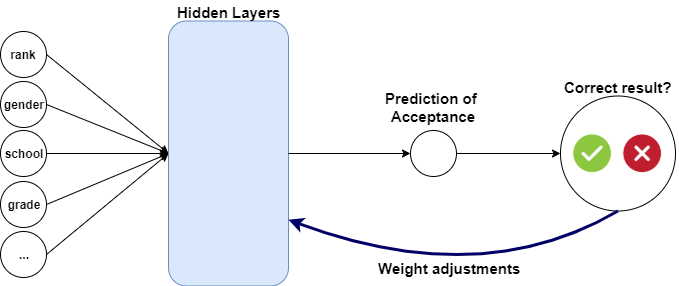
\includegraphics[width=350pt]{images/neuralNetwork.png}
                \caption{A visual of the architecture used in the deep learning approach}
                \label{fig:nnApproach}
            \end{figure}
        
        \newpage
        
        \subsubsection{SVM Approach}
        
        % brief description of what this approach typically consists of
        % why we chose this approach
        % how it applies to our data and purpose
        % how it'll work for us
        
        As in the machine learning approach, the purpose of the support vector machine approach is to essentially classify the data into one of two classes: a class where the students will accept the offer, and the other where they won't.
        \textbf{Support vector machines (SVMs)} are a supervised machine learning approach to determine an optimal hyperplane for data classification when the data is visualized in multiple dimensions. 
        For our application, a kernelized SVM may be used to obtain increased accuracy, wherein functions called \textbf{kernel tricks} will use dot products to map data points into higher dimensions to transform non-linear data into linear space and improve classification accuracy.
        
        Since speed is not a requirement for this project, the potential drawback that comes with using SVMs leading to larger processing times  is superficial\footnotemark. 
        Be that as it may, as mentioned earlier, kernel functions, as well as tuned hyperparameters, will be incorporated to increase speed.
        
        One of the reasons why the SVM is considered a viable approach for this project is because SVMs are effective in high dimension spaces\footnotemark[\value{footnote}] and in this classification process, multiple dimensions result from the multiple features that must be considered for each student.
        
        \footnotetext{See source: https://towardsdatascience.com/support-vector-machines-svm-c9ef22815589}
        
        The steps that will be taken to implement this approach can be broken down into 3 main steps as listed below:
        
        \begin{enumerate}
            \item Start with data that the model will be trained using (as outlined in \underline{\ref{cutoffMetDataCleaning}}).
            \begin{itemize}
                \item As with the deep learning approach, data will be input as feature vectors.
                \item Within the implementation, the decision boundary will be drawn arbitrarily at first, and will continue to improve once more data is passed through the learning model.
            \end{itemize}
            \item ``Transform'' data to higher dimensions to optimize accuracy of decision boundary.
                \begin{itemize}
                    \item Data will be transformed into higher dimensional spaces to allow for optimal accuracy for the determined hyperplane, using the aforementioned ``kernel trick" to reduce computational costs as much as possible.
                    \item Part of the development process includes manipulating kernel types to see how the model can best be improved in terms of accuracy. Some popular kernel types include polynomial kernels, RBF kernels, sigmoid kernels, etc.. Tuning will likely be required for the kernel parameters as well.
                \end{itemize}
            \item Find the support vector classifier that classifies higher dimensional data into 2 groups by continuously validating and optimizing the found hyperplanes.
        \end{enumerate}
        
        Due to the assumption that the data is likely well-behaved enough to determine a trend, not too many outliers and extreme examples are expected, however, in the case of such outliers, a soft-margin approach will allow the model some misclassification for the sake of optimizing classification in the long run.
        Part of the task is to research and tweak parameters to optimize bias/variance tradeoff for our application.
        Through training, the model should be able to draw a decision boundary with some margin from the potential extreme points in either classified group to allow for optimal classification by taking into account potential outliers in the data.
        
        \subsection{Limitations}
        Some potential limitations of the proposed system are outlined as follows.
        \subsubsection{Size of Dataset}
        One major limitation that must be considered is the relatively small size of our dataset. Our training data contains data for just 7 admissions cycles and for each of these cycles only data for students that received an offer are pertinent. The concern with this is that of overfitting. When training data is limited, the resulting model may not be as robust or general and instead correspond too closely to the data it was trained with. 
        This can be reconciled however by taking into consideration that in general we expect future admissions cycles to be quite similar to the ones we are training with. 
        Our application is one for which we do not expect many edge cases or noise.
        
        \subsubsection{Computation Efficiency}
        In general, when talking about machine learning approaches a major limitation is the amount of time and computation power needed. 
        Since our dataset is smaller and constant in size this is a secondary concern.
        The focus will be on the accuracy of the system rather than its speed or efficiency.
        
        \subsection{Software Architecture}
        The following describes a primitive outline of the software architecture we will follow: \\
        
        \begin{center}
        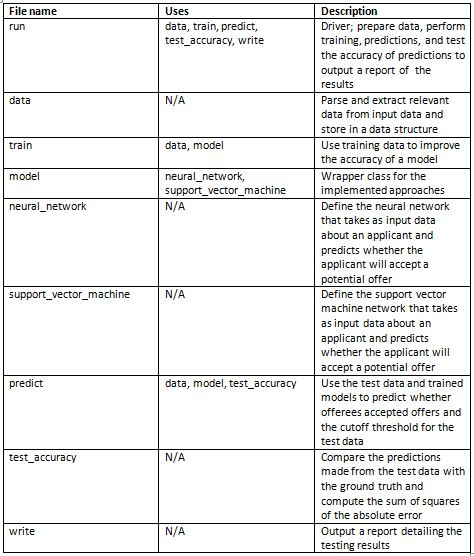
\includegraphics[width=400pt]{images/architectureTable.JPG}
        \end{center}
        
        \begin{center}
        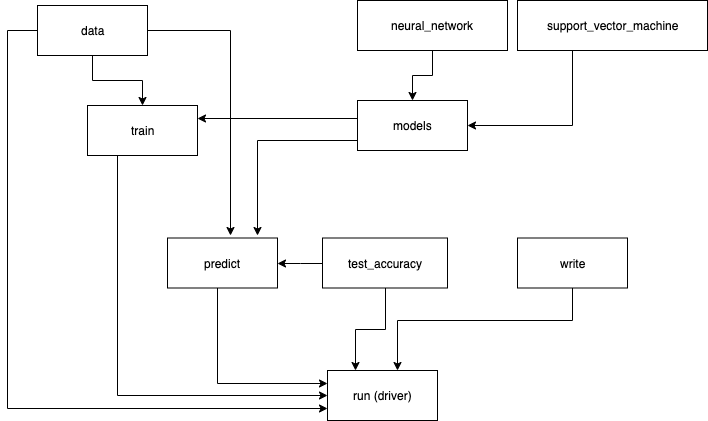
\includegraphics[width=400pt]{images/architectureFlowchart.png}
        \end{center}

    \newpage

	\section{User Interface}
	The system will involve little user interaction and as such will be delivered in the form of a command-line application. 
	It is intended that the system will be run on MAC, Linux/Unix and Windows operating systems.
	Users will be required to upload the data they would like to input to the system in a specified input directory and format. 
	The application will then use the data and run it through the system to output a result directly to the terminal/command prompt describing the GPA cutoff threshold predicted by the system, how many offers to be sent out, and how many offerees are predicted to accept the offer. 
	Additional files will be created with further information about the results and be stored in a specified output directory.

    \section{Milestones}
    The following describes a general outline of the milestones our project is divided into: \\
    \begin{center}
    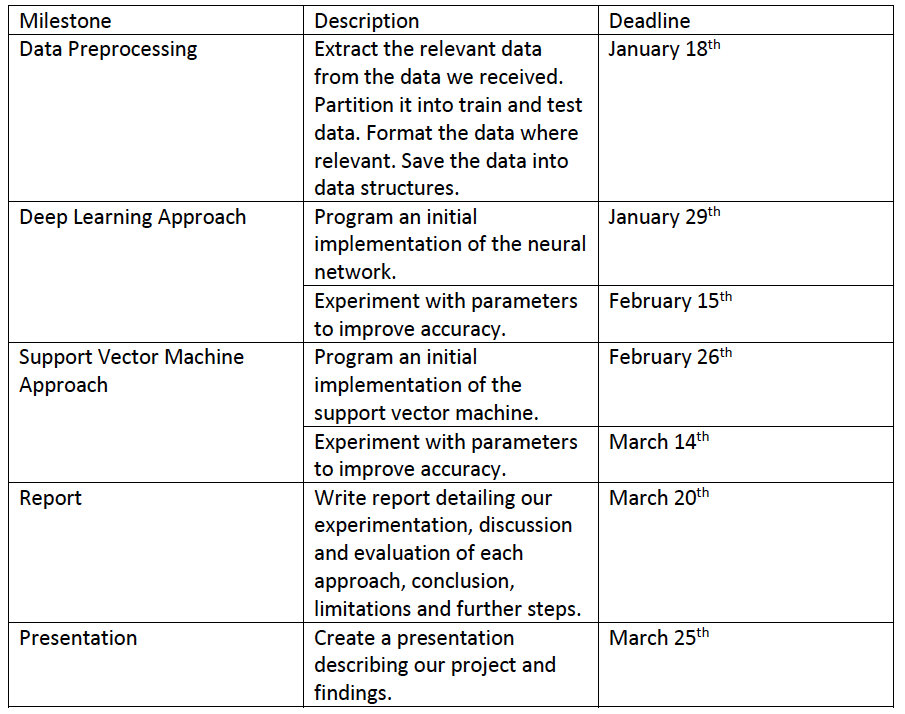
\includegraphics[width=400pt]{images/milestones.png} 
    \end{center}
    Note: as majority of our project is experimentation in an attempt to improve the accuracy of our models, it does not very closely follow the traditional milestones and architecture of software projects.

\end{normalsize}
\end{document}
